\documentclass{acmsmall}
\usepackage{siunitx}
\usepackage{booktabs}
\usepackage{url}
\usepackage[ruled]{algorithm2e}
\renewcommand{\algorithmcfname}{ALGORITHM}
\SetAlFnt{\small}
\SetAlCapFnt{\small}
\SetAlCapNameFnt{\small}
\SetAlCapHSkip{0pt}
\IncMargin{-\parindent}


\newcommand{\dmcomment}[1]{\textbf{#1}}


\begin{document}

\title{Replicated Computational Results (RCR) Report for
  ``A distributed-memory package for dense Hierarchically
    Semi-Separable matrix computations using randomization''}

\author{Dominic Meiser
\affil{Tech-X Corporation, 5621 Arapahoe Avenue, Boulder CO, 80303, USA.}
}

\newcommand{\strumpack}{STRUMPack}

\begin{abstract}
  In this report we replicate a subset of the performance results
  in the paper ``A distributed-memory package for dense
  Hierarchically Semi-Separable matrix computations using
  randomization''.
\end{abstract}

\maketitle 

\section{Introduction}

Rouet et al. present details of a newly developed library,
\strumpack{}, for the construction of hierarchically
semi-separable matrices and for arithmetic with these
matrices~\cite{rouet:strumpack}.  Among other things,
\strumpack{} provides facilities to convert ordinary dense
matrices into a hierarchical matrix format.  Compression is
achieved by means of a low rank approximation for sub blocks of
the matrix.  \strumpack{} provides functions to factor the
resulting hierarchical matrix into a form suitable for efficient
solution and thus provides a means to create pre-conditioners for
dense matrix problems.  All of this functionality is available in
a distributed memory architecture based on MPI.

In this report we replicate a representative subset of the
computational results presented by Rouet et al.  We focus on
compression, factorization, and solver performance reported in
Table III of~\cite{rouet:strumpack}.  We also replicate the
strong scaling results reported in~Fig.~10
in that paper.

Specifically, we carry out the following steps:
\begin{enumerate}
  \item Download the \strumpack{} distribution package.
  \item Build \strumpack{} on a laptop.
  \item Build \strumpack{} on Edison at NERSC.
  \item Run \strumpack{} on Edison to replicate performance
    measurements for QChem Toeplitz matrix and to check strong
    scaling for a dense matrix from a boundary element formulation
    of an electromagnetic scattering problem.
\end{enumerate}

The following sections provide details on these steps.


\section{Building \strumpack{} on a laptop}

To verify that we could build the package we first get it to run
on a laptop.  This allows us to iron out any issues ahead of time
in an environment that we have complete control over before
attempting to do the same on an expensive computer like Edison.
Additionally, this provides confidence that \strumpack{} can be
used on generic computers and not just in the specific
environment used by Rouet et al.

We obtain the sources from the \strumpack{} distribution website,
\begin{verbatim}
STRUMPACK_URL=http://portal.nersc.gov/project/sparse/strumpack \
  TARBALL_NAME=STRUMPACK-Dense-1.1.1.tar.gz \
  wget $STRUMPACK_URL/$TARBALL_NAME
tar xf STRUMPACK-Dense-1.1.1.tar.gz
\end{verbatim}

The source distribution contains a 20 page manual with
introduction, installation instructions, background on the
algorithms, and an API reference.  A readme file
provides concise instructions on how to build \strumpack{}.

\strumpack{}'s third party library requirements are rather
minimal: MPI, BLAS, LAPACK, and ScaLAPACK.  For our laptop builds
We satisfy these requirements as follows:
\begin{itemize}
\item For MPI we use mpich version 3.1.4.
\item For BLAS and LAPACK we use the binary distribution on
the centos 6 linux distribution (rpm packages
\verb!blas-3.2.1-4.el6.x86_64!,
\verb!blas-devel-3.2.1-4.el6.x86_64!,
\verb!lapack-3.2.1-4.el6.x86_64!, and
\verb!lapack-devel-3.2.1-4.el6.x86_64!).
\item For ScaLAPACK we use version 2.0.2 from netlib~\cite{netlib}.
\end{itemize}
All code is compiled with gcc version 4.9.3.

\strumpack{}'s build system consists of gnu makefiles.  The
makefiles are
customized by writing a Makefile.inc that defines system specific
variables.  Examples of Makefile.inc files are provided for gnu
based linux systems, Edison, and Hopper.  To build on our laptop
we modify Makefile.gnu to point to our MPIO, BLAS, LAPACK, and
ScaLAPACK installation.  With these modifications we successfully
build the C++, C, and Fortran examples.  We don't verify building
of the matlab bindings because our laptop does not have matlab
installed.  We are able to execute all example binaries and the
output from them looks plausible.


\section{Building on Edison}

The majority of the performance results reported
in~\cite{rouet:strumpack} were obtained on Edison~\cite{Edison} at
NERSC.\@ To build \strumpack{} on Edison we use the default intel
programming environment, \verb!PrgEnv-intel/5.2.56!  with version
15.0.1 20141023 of the intel compilers, and with module
\verb!cray-mpich/7.3.1! for MPI support.  The template
\verb!Makefile.edison! provided with the source distribution of
STRUMPACK works without modifications with these modules.  The
Makefile.edison file compiles all sources with \verb!-O3!.


\section{Performance on Edison}

We use the example \verb!solve.cpp! to reproduce the results for
the QChem Toeplitz matrices in Table~III
in~\cite{rouet:strumpack}.  Currently there is no mechanism to
control the example program via command line options.  Thus we
modify the \verb!solve.cpp! source code and rebuild for every set
of parameters.  We set the problem size to \verb!n=80,000! and
change the number of right hand sides to \verb!nrhs=1!.  Details
of the computation are controlled via options of the
computational object \verb!sdp! of type
\verb!StrumpackDensePackage!.  After discussion with Rouet et
al.\ we configure \verb!sdp! as follows to match the settings used
in~\cite{rouet:strumpack}:
\begin{verbatim}
sdp.use_HSS=true;
sdp.tol_HSS=1e-8;
sdp.levels_HSS=13;
sdp.min_rand_HSS=250;
sdp.lim_rand_HSS=5;
sdp.inc_rand_HSS=10;
sdp.max_rand_HSS=250;
sdp.steps_IR=10;
sdp.tol_IR=1e-8;
\end{verbatim}
The setting \verb!sdp.use_HSS=true! specifies that HSS
compression be used.  By setting this parameter to false it is
possible to test the solution of the system via ScaLAPACK instead
of \strumpack{}.  The parameter \verb!sdp.tol_HSS! sets
$\epsilon$ in Table III in~\cite{rouet:strumpack}.  The parameter
\verb!sdp.levels_HSS! specifies the maximum number of levels in
the HSS tree.  The parameters \verb!sdp.min_rand_HSS!,
\verb!sdp.lim_rand_HSS!, \verb!sdp.inc_rand_HSS!, and
\verb!sdp.max_rand_HSS! configure the adaptive sampling of random
vectors used for the construction of the HSS matrix in
\strumpack{}.  By setting minimum and maximum numbers of random
vectors equal to one another,
\verb!sdp.min_rand_HSS==sdp.max_rand_HSS!, we effectively disable
the adaptive sampling algorithm and use a fixed number of
vectors, 250 in the example above.  The number of sampling
vectors is adjusted for the different tolerances $\epsilon$ since
the maximum rank depends on the precision of the reduced rank
representation.  The number of sampling vectors is indicated in
table~\ref{table:QChemToeplitz} for each $\epsilon$.  The
parameter \verb!sdp.steps_IR! determines the maximum number of
iterations used for iterative refinement and \verb!sdp.tol_IR!
specifies the precision to which the linear system is being
solved.  Reporting of performance numbers relies on the
function \verb!sdp.print_statistics()!.

Initially we run the \verb!solve! driver in a mode where the
precision of the compressed matrix is verified.  The verification
of the compression is a very memory intensive operation and thus
requires more compute nodes than were used
in~\cite{rouet:strumpack}.  After successfully verifying the
accuracy of the compression we disable the verification feature
and reduce the number of nodes to the configuration used
in~\cite{rouet:strumpack}.  Specifically, we use four compute
nodes with 16 MPI processes on each of them.

Our performance results are shown in
table~\ref{table:QChemToeplitz} along with the results reported
in~\cite{rouet:strumpack} for comparison.  The timings we obtain
for the compression step are very close to the results reported
in~\cite{rouet:strumpack}.  The timings for factorization and
solution vary a bit.  But because these stages are only fractions
of a second long they are much more susceptible to fluctuations.
In our estimation the timing results are close enough to consider
the results of~\cite{rouet:strumpack} replicated.
\begin{table}
  \tbl{Summary of performance measurements.  All numbers indicate
    times in seconds.  The timings from~\cite{rouet:strumpack} are
    indicated in parenthesis.  The column labeled \# Rand.\ Vecs
    indicates the number of sampling vectors used for the
    compression, Max.\ rank indicates the maximum rank for any
    sub-block estimated by \strumpack{} for the given level of
    accuracy, Compression lists the times consumed for HSS
    compression, Factorization the time for computing the ULV
    factorization of the compressed matrices, and Solution + IR is
    the time for solution and iterative refinement.  All times are in
    seconds.}{
  \begin{tabular}{cccccc}
\toprule
$\epsilon$ & \# Rand.\ Vecs & Max.\ rank & Compression & Factorization & Solution + IR\\
\midrule
    \SI{1.0e-8} & 250 & 171 (169) & 19.0 (19.0) & 0.04 (0.04) & 0.2 (1.5)\\
    \SI{1.0e-6} & 200 & 147 (147) & 18.2 (17.6) & 0.07 (0.03) & 0.7 (2.0)\\
    \SI{1.0e-4} & 150 & 121 (120) & 16.9 (16.7) & 0.04 (0.02) & 0.4 (5.6)\\
\bottomrule
  \end{tabular}
    }
\label{table:QChemToeplitz}
\end{table}
\dmcomment{Sherry, Fran\c{}cois, I think I'm getting very different
  times for the solution step because I'm solving to a smaller
  accuracy (sdp.tol\_IR in the code).  I use
  sdp.tol\_IR=sdp.tol\_HSS.  What should I use for sdp.tol\_IR?}

Besides the timing results we also made sure that the maximum
rank reported by \strumpack{} agrees with~\cite{rouet:strumpack}.
We find that in our runs the maximum rank is within 1\% of the
ranks reported in~\cite{rouet:strumpack}.  The maximum rank
obtained depends on the random sampling vectors.  As the sampling
vectors are not identical from run to run it is not surprising
that there are small variations.


\section{Replication of strong scaling results}

To replicate the strong scaling performance reported in Fig.~10
in~\cite{rouet:strumpack} we use the program, \verb!driver.cpp!,
that was used by Rouet et al for that study.  This executable is
not part of the release distribution of~\cite{rouet:strumpack}.
We build it on Edison using
\begin{verbatim}
CC driver.cpp -I ${STRUMPACK_SRC_DIR}
\end{verbatim}
The directory \verb!STRUMPACK_SRC_DIR! is the directory in which
the \strumpack{} sources are located.  The driver program loads
the matrices from Rouet's scratch directory on Edison.  The
matrices are stored in a proprietary binary format.

The timing results for the different stages of the solution
process are shown in Fig.~\ref{fig:strongscaling}.  For this run
we use 6000 random vectors for the random sampling space and the
depth of the HSS tree is 6.  The equations are solved to a
precision of $\epsilon=$\SI{1.0e-4}.  We use the timing
measurements as reported by \verb~driver.cpp~.  While we are not
sure how to compute the total solution times reported
in~\cite{rouet:strumpack} from the application logs, our results
are at least in qualitative agreement.  The compression,
factorization, and matrix vector multiplication strong scale well
to 2048 MPI process.  The solution kernel does not scale well
which is not surprising given the small amount of parallelism
that can be exploited by this computation.
\begin{figure}
  \begin{center}
  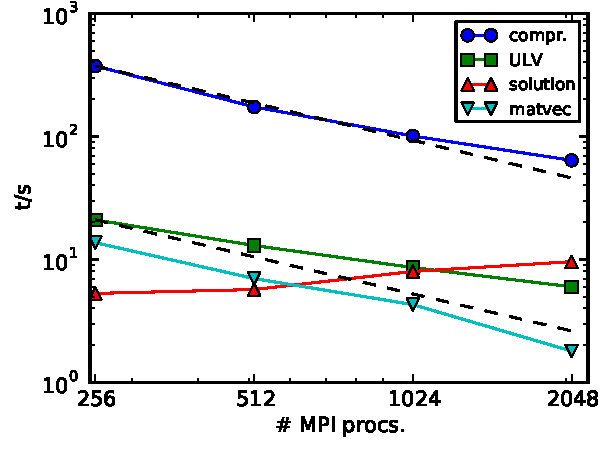
\includegraphics[width=0.5\textwidth]{strong_scaling}
  \end{center}
  \caption{Strong scaling of various stages of the solution of an
  electromagnetic boundary element problem with \strumpack{}.
  ``compr.'' refers to the HSS compression, ``ULV'' to the
  factorization,  and ``solution'' and ``matvec'' are statistics
  for the solution stage and matrix vector products.}
  \label{fig:strongscaling}
\end{figure}


\section{Conclusion}

We replicate the results reported in~\cite{rouet:strumpack}.  The
STRUMPACK library is easy to build and contains sufficient
documentation for others to use the library.  We build the
library on a laptop and on Edison.  We reproduce the timing
results reported for a synthetic matrix as well as strong scaling
results for a matrix originating from an electromagnetic boundary
element problem.


\section{Acknowledgements}

We would like to thank Fran\c{}ois-Henry Rouet and Xiaoye S. Li for
valuable feedback and discussion and M. Heroux for guidance.
This research used resources of the National Energy Research
Scientific Computing Center, which is supported by the Office of
Science of the U. S. Department of Energy under Contract No. ???
\dmcomment{Hi Sherry, what contract should I acknowledge for
mp127 time? Thanks.}

\bibliographystyle{abbrv}
\bibliography{strumpack}

\end{document}
